\documentclass{article}

\usepackage{amsmath}
\usepackage[usenames,dvipsnames]{color}
\usepackage{multirow}
\usepackage{listings}
\usepackage[a4paper, top=2cm, bottom=3cm, left=4cm, right=4cm]{geometry}

\usepackage{tikz}
\usetikzlibrary{shapes, shapes.multipart, shapes.geometric}
\usetikzlibrary{positioning}

\newcommand*\circled[1]{\tikz[baseline=(char.base)]{
            \node[shape=circle,draw,inner sep=2pt] (char) {#1};}}

\begin{document}

\section{Method}

\begin{figure}[ht]
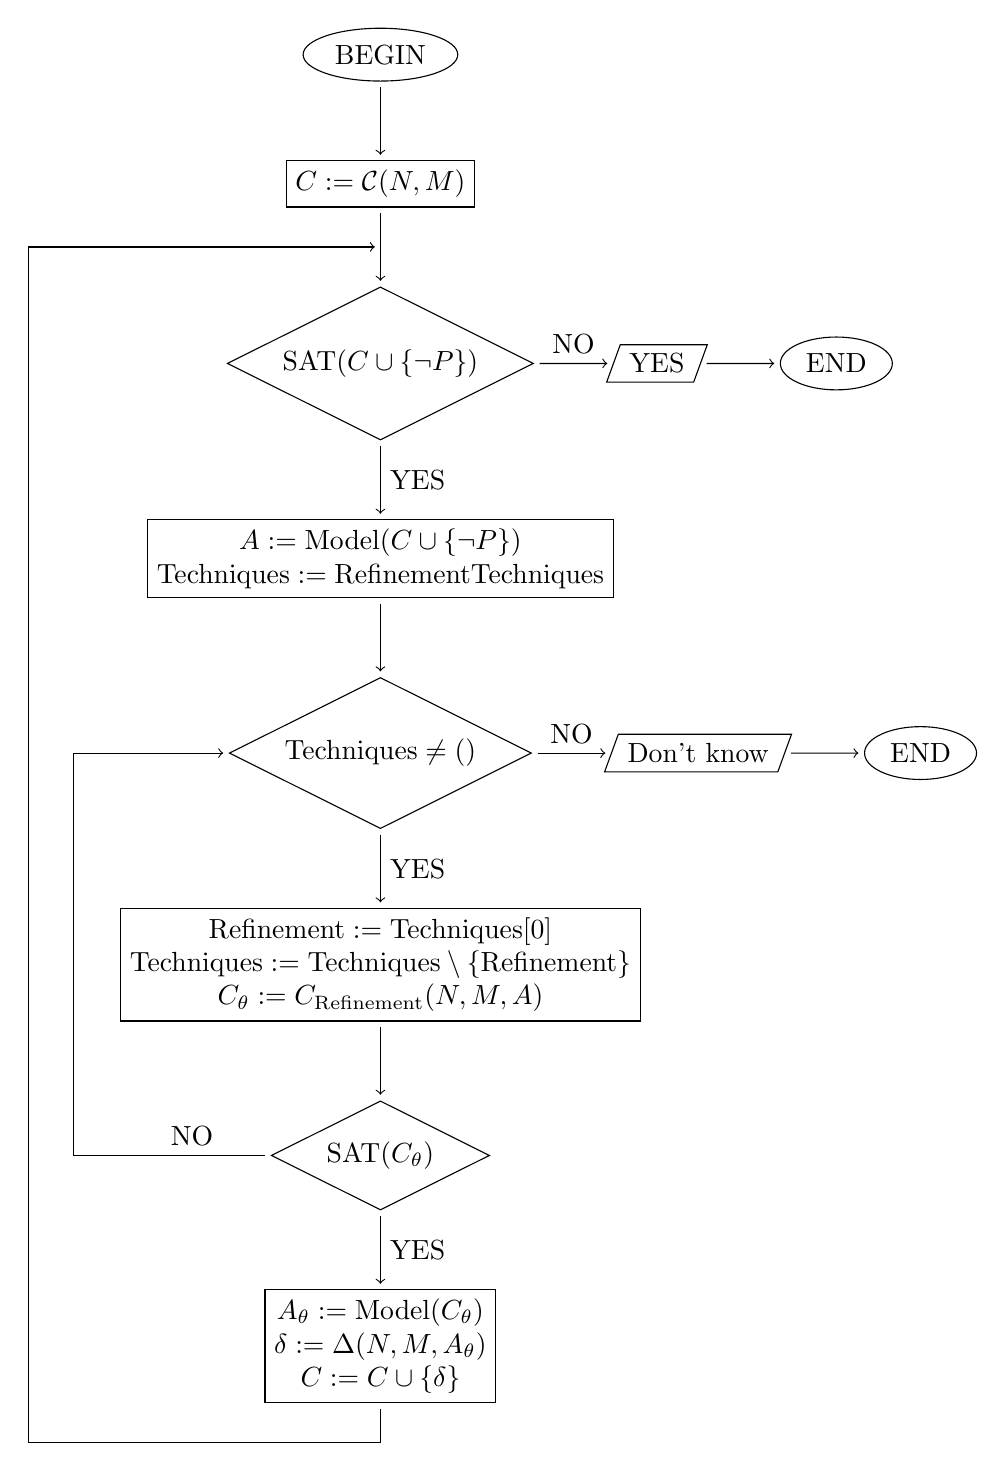
\begin{tikzpicture}[
    state/.style   = {draw, ellipse, aspect=2},
    action/.style  = {draw, rectangle, align=center},
    decision/.style= {draw, diamond, aspect=2, align=center},
    print/.style   = {draw, trapezium, trapezium left angle=70, trapezium right angle=-70},
    edge/.style    = {draw, ->, shorten >=2pt, shorten <=2pt},
  ]
  \node[state] (begin) {BEGIN};
  \node[action, below=of begin] (c) {$C:=\mathcal C(N, M)$};
  \node[decision, below=of c] (satc) {$\text{SAT}(C \cup \{\neg P\})$};
  \node[action, below=of satc] (modelc)
    {$A:=\text{Model}(C \cup \{\neg P\})$ \\
     $\text{Techniques}:=\text{RefinementTechniques}$};
     \node[decision, below=of modelc] (methods) {$\text{Techniques} \neq ()$};
  \node[action, below=of methods] (ctheta)
    {$\text{Refinement} := \text{Techniques}[0]$ \\
     $\text{Techniques}:= \text{Techniques} \setminus \{\text{Refinement}\}$ \\
     $C_{\theta}:=C_{\text{Refinement}}(N, M, A)$};
  \node[decision, below=of ctheta] (satctheta) {$\text{SAT}(C_\theta)$};
  \node[action, below=of satctheta] (modelctheta)
    {$A_\theta:=\text{Model}(C_\theta)$\\
     $\delta:=\Delta(N, M, A_\theta)$\\
     $C:=C \cup \{\delta\}$};
  \node[print, right=of satc] (yes) {YES};
  \node[state, right=of yes] (end1) {END};
  \node[print, right=of methods] (dontknow) {Don't know};
  \node[state, right=of dontknow] (end2) {END};

  \draw (begin) edge[edge] (c);
  \draw (c) edge[edge] coordinate[pos=.5] (edgein) (satc);
  \draw (satc) edge[edge] node[above]{NO} (yes);
  \draw (yes) edge[edge] (end1);
  \draw (satc) edge[edge] node[right]{YES} (modelc);
  \draw (modelc) edge[edge] (methods);
  \draw (methods) edge[edge] node[right]{YES}  (ctheta);
  \draw (methods) edge[edge] node[above]{NO} (dontknow);
  \draw (ctheta) edge[edge] (satctheta);
  \draw (dontknow) edge[edge] (end2);
  \draw (satctheta) edge[edge] node[right]{YES} (modelctheta);
  \draw[edge] (satctheta.west) node[above,xshift=-1cm]{NO}
  -| ([xshift=-2.5cm] satctheta.west) |- (methods.west);
  \draw[edge] (modelctheta.south) -- ([yshift=-0.5cm] modelctheta.south)
  -| ([xshift=-3cm] modelctheta.west) |- (edgein);
\end{tikzpicture}
\caption{The method}
\label{fig-method}
\end{figure}

\newpage

\section{Benchmarks}

\subsection{Given by Daniel Kroening}

\begin{table}[h]
\begin{center}
  \begin{tabular}{ | p{6cm} | r | r | r | r | }
    \hline
    Method & positive & negative & don't know & timeout \\
    \hline
    M1: State equation with real numbers & 23 &  0 & 54 &  0 \\
    M2: State equation with integers     & 23 &  0 & 54 &  0 \\
    \hline
    M3: M2 with TrapConditions               & 23 &  0 & 54 &  0 \\
    M4: M3 with SubnetTrapConditions         & 23 &  0 & 50 &  4 \\
    M5: M4 with EmptyTrapConditions          & 23 &  0 & 46 &  8 \\
    \hline
    M6: M1 with State space exploration, timeout of  1\,min & 26 & 34 & 0 & 17 \\
    M7: M1 with State space exploration, timeout of 10\,min & 26 & 39 & 0 & 12 \\
    M8: M1 with State space exploration, timeout of  8\,h   & 26 & 45 & 0 &  6 \\
    \hline
    M9: Bfc tool  & 26 & 51 & 0 &  0 \\
    \hline
  \end{tabular}
\end{center}
\caption{Compiled results of the benchmarks given by Daniel Kroening}
\label{table-results-compiled-dk}
\end{table}

Positive files for method 1:
\begin{lstlisting}
cprover-PN/abp
cprover-PN/basicME
cprover-PN/bingham_h150
cprover-PN/bingham_h25
cprover-PN/bingham_h250
cprover-PN/bingham_h50
cprover-PN/bingham_h500
cprover-PN/clientserver
cprover-PN/csm
cprover-PN/gsm
cprover-PN/handover
cprover-PN/keycard
cprover-PN/mesh2x2
cprover-PN/multipoll
cprover-PN/newrtp
cprover-PN/phones
cprover-PN/reaction
cprover-PN/reaction3
cprover-PN/reaction4
cprover-PN/read-write
cprover-PN/restriction
cprover_software_analysis/conditionals_vs_satabs.2/main
cprover_software_analysis/rand_cas_vs_satabs.2/main
\end{lstlisting}

Additional positive files for method 6:
\begin{lstlisting}
cprover-PN/lamport
cprover-PN/newdekker
cprover-PN/peterson
\end{lstlisting}

\newpage

\subsection{Found in mist repository}

\begin{table}[h]
\begin{center}
  \begin{tabular}{ | p{6cm} | r | r | r | r | }
    \hline
    Method & positive & negative & don't know & timeout \\
    \hline
    M1: State equation with real numbers & 16 &  0 & 11 &  0 \\
    M2: State equation with integers     & 16 &  0 & 11 &  0 \\
    \hline
    M3: M2 with TrapConditions               & 20 &  0 &  7 &  0 \\
    M4: M3 with SubnetTrapConditions         & 21 &  0 &  6 &  0 \\
    M5: M4 with EmptyTrapConditions          & 21 &  0 &  6 &  0 \\
    \hline
    M10: M4 with State space exploration, timeout of 4\,h & 21 &  2 & 0 &  4 \\
    \hline
    M11: Mist tool & 23 &  4 & 0 &  0 \\
    \hline
  \end{tabular}
\end{center}
\caption{Compiled results of the benchmarks found in mist repository}
\label{table-results-compiled-mist}
\end{table}

Positive files for method 1:
\begin{lstlisting}
PN/MultiME
PN/basicME
PN/bingham_h150
PN/bingham_h25
PN/bingham_h250
PN/bingham_h250_attic
PN/bingham_h50
PN/csm
PN/fms
PN/fms_attic
PN/mesh2x2
PN/mesh3x2
PN/multipool
boundedPN/kanban
boundedPN/newrtp
boundedPN/read-write
\end{lstlisting}

Additional positive files for method 3:
\begin{lstlisting}
PN/pingpong
boundedPN/lamport
boundedPN/newdekker
boundedPN/peterson
\end{lstlisting}

Additional positive files for method 4:
\begin{lstlisting}
PN/manufacturing
\end{lstlisting}

Additional positive files for method 11:
\begin{lstlisting}
PN/extendedread-write
PN/extendedread-write-smallconsts
\end{lstlisting}

\end{document}
